\documentclass[14pt]{extreport}

\usepackage{gost}
\usepackage{listings}
\usepackage{longtable,rotating}
\usepackage{threeparttable}
\usepackage{amsmath}

\begin{document}

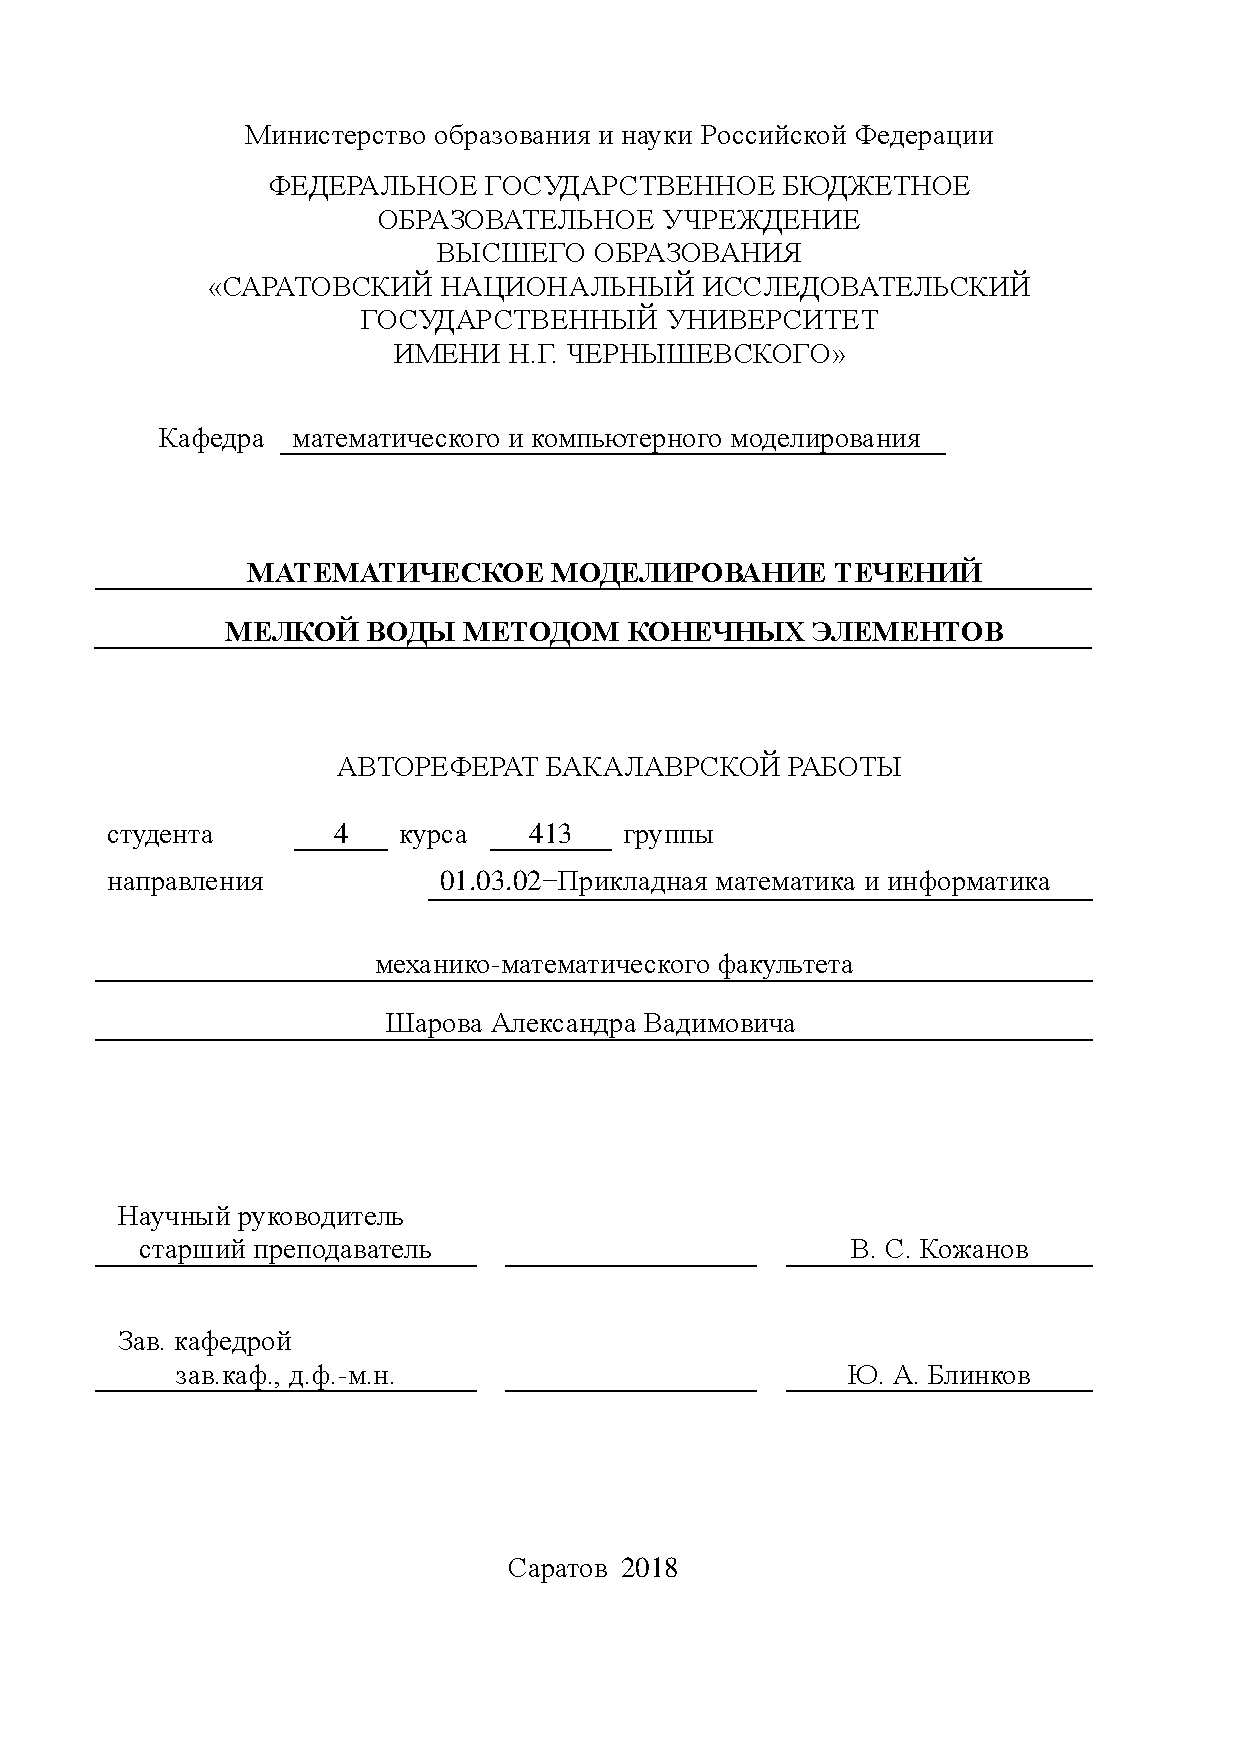
\includepdf[pages={1}]{titul/report.pdf}

\tableofcontents
\intro

На данный момент во многих случаях не оправдывается применение более сложных математических моделей для исследования течений в прибрежных водах и озерах, чем моделей, основанных на численном решении двумерных уравнений, полученных путем применения осредненных по вертикали характеристик - уравнений мелкой воды. Трехмерные решения нецелесообразны, так как они требуют намного большего количества исходной информации и машинного времени даже с учетом современных вычислительных мощностей.


\chapter{Общая структура работы}
\section{Актуальность работы}
Актуальность данной работы обусловлена тем, что со второй половины 20-го века метод математического моделирования стал рабочим инструментом при изучении многих научно-технических задач, в частности, и в области гидродинамики. Основной составляющей этого метода стал является вычислительных эксперимент, широкое применение которого стало возможным благодаря развитию производительности ЭВМ и численных алгоритмов. Вычислительный эксперимент позволяет получить информацию о структуре течения при относительно небольших временных, трудовых и материальных затратах. конечно, при этом соответствующая математическая модель должна быть адекватной физическому процессу.


\section{Цели и задачи работы}
Целью представленной выпускной квалификационной работы является осуществление математического моделирования течений мелкой воды с помощью метода конечных элементов, который уже давно зарекомендовал в таких областях как механика деформируемого тела, электродинамика и конечно же гидродинамика. Данный метод является оптимальным для решения поставленной задачи так как именно он дает возможность применять достаточно гибкую разбивку рассматриваемой области и при его использовании достаточно удовлетворить лишь главным граничным условиям.

\section{Практическая значимость}
В данной дипломной работе получены следующие теоретические и практические результаты

\begin{enumerate}
\item сформулированна задача движения мелкой воды в закрытом водоеме
\item решена задача триангуляции реальных озер и написана программная реализация
\item написана программная реализация для расчета математической модели движения мелкой воды с помощью метода конечных элементов
\item проведены эксперименты на различных типах прудов и озер
\end{enumerate}




 позволяют рассчитать и продемонстрировать движение мелкой воды в закрытом водоеме.


\chapter{Содержание бакалаврской работы}


\section{Вывод уравнений мелкой воды}

Уравнения мелкой воды выводятся из двух основных уравнений для жидкости, а именно уравнения количества движения и уравнения неразрывности:

\begin{equation}\label{eq:shallow_water:1}
-\frac{\partial p}{\partial x_k} + \frac{\partial \tau_{ik}}{\partial x_i} + \rho b_k = \frac{\partial}{\partial x_i}(\rho v_i v_k) + \frac{\partial}{\partial t}(\rho v_k);
\end{equation}

\begin{equation}\label{eq:shallow_water:2}
\frac{D\rho}{Dt}+\rho \frac{\partial v_i}{\partial x_i} =0
\end{equation}

При математическом моделировании движения мелкой воды сложно применять данные уравнения из-за наличия свободной поверхности, изменения границ во время приливов и отливов и вследствие большого количества переменных.

Данных трудностей можно избежать после ряда упрощений, в результате чего получается уравнения мелкой воды:

\begin{equation}\label{eq:shallow_water:22}
\begin{aligned}
\frac{\partial q_1}{\partial t} + \frac{\partial}{\partial x_1} \bigg(\frac{q_1^2}{H}\bigg)+\frac{\partial }{\partial x_2}\bigg(\frac{q_1 q_2}{H}\bigg) = \frac{\partial}{\partial x_1} (N_{11}-N_p) + \frac{\partial N_{12}}{\partial x_2} + B_1; \\
\frac{\partial q_2}{\partial t} + \frac{\partial}{\partial x_1} \bigg(\frac{q_1 q_2}{H}\bigg)+\frac{\partial }{\partial x_2}\bigg(\frac{q_2^2}{H}\bigg) = \frac{\partial}{\partial x_2} (N_{22}-N_p) + \frac{\partial N_{12}}{\partial x_2} + B_2,
\end{aligned}
\end{equation}

\noindentгде

\begin{equation}\label{eq:shallow_water:23}
\begin{aligned}
B_1=fq_2+\gamma^2\rho_aW^2\cos(\theta)-\bigg(\frac{g}{c^2}\bigg)\frac{1}{\rho}\frac{q_1\sqrt{(q_1^2+q_2^2)}}{H^2} + p_a \frac{\partial H}{\partial x_1} + \rho gH\frac{\partial h}{\partial x_1}; \\
B_2=-fq_1+\gamma^2\rho_aW^2\sin(\theta)-\bigg(\frac{g}{c^2}\bigg)\frac{1}{\rho}\frac{q_2\sqrt{(q_1^2+q_2^2)}}{H^2} + p_a \frac{\partial H}{\partial x_2} + \rho gH\frac{\partial h}{\partial x_2}.
\end{aligned}
\end{equation}


\section{Триангуляция двумерной области}

В геометрии триангуляция дискретного множества точек $P\subset {\mathbb  {R}}^{{n+1}}$ в наиболее общем значении — это разбиение  выпуклой оболочки некоторого набора точек, которое представляет собой планарный граф. Одна из фигур разбиения является выпуклой оболочкой разбиваемого множества, а остальные - симплексами -  геометрическими фигурами, которые являются $n-$мерным обобщением треугольника. В любой триангуляции ($T$) формально должны выполняться следующие свойства:

	1. любые два симплекса в T пересекаются в общей грани ребра или вершины, или вообще не пересекаются;

	2. множество точек, являющихся вершинами симплексов разбиения, совпадает с множеством $P$;
	
	3. нельзя добавить ни одного нового ребра в граф без нарушения планарности.

Одно и то же множество можно триангулировать разными способами. Триангуляция дает тем лучшую аппроксимацию, чем больше её минимальный угол, при этом формируемые симплексы стремятся к равноугольности. Очень важна максимизация минимального угла в вычислительных задачах, когда точность производимых вычислений очень сильно зависит от размера минимального угла триангуляции. Наилучшей в этом смысле триангуляцией является триангуляция Делоне. Простейшим способом её построения является инкрементальный алгоритм, работающий за $o(n^2)$ операций, но он не поддерживает вырожденные случаи, когда 4 точки из множества лежат на одной окружности: в этом случае триангуляция Делоне не уникальна, и способов разбиения существует несколько, но минимальные углы этих триангуляций равны. Иногда даже минимальный угол триангуляции Делоне оказывается слишком малым для устойчивой работы использующего её алгоритма, и тогда можно произвести улучшение, используя метод Рапперта [J. Ruppert]. При этом будут добавлены новые вершины триангуляции, а так же образованы дополнительные треугольники. Стабильность численного алгоритма (метода конечных элементов, к примеру) может возрасти многократно за счет появления нижней границы для углов. 

\section{Метод конечных элементов в двумерной области}

Метод конечных элементов \cite{bib:fem:pankratov, bib:fem:zenkevich} - численный метод решения дифференциальных уравнений с частными производными, возникающими при решении задач прикладной физики.
	В его основе лежат две главные идеи: дискретизация исследуемого объекта и кусочно-элементная аппроксимация исследуемых функций(в физической интерпретации - температуры, давления, перемещения и т.д.).

Идея состоит в том, что область, в которой ищется решение дифференциальных уравнений, разбивается на конечное количество элементов. В каждом из элементов произвольно выбирается вид аппроксимирующей функции. Вне своего элемента аппроксимирующая функция равна нулю. Значения функций в узлах являются решением задачи и заранее неизвестны. Коэффициенты аппроксимирующих функций обычно ищутся из условия равенства значения соседних функций на границах между элементами (в узлах). Затем эти коэффициенты выражаются через значения функций в узлах элементов. Составляется система линейных алгебраических уравнений. Количество уравнений равно количеству неизвестных значений в узлах, на которых ищется решение исходной системы, прямо пропорционально количеству элементов. Так как каждый из элементов связан с ограниченным количеством соседних, система линейных алгебраических уравнений имеет разрежённый вид, что существенно упрощает её решение. 


В рассматриваемой системе \ref{eq:task:1}-\ref{eq:task:2} можно пренебречь членами $-fq_{1}$ и $fq_2$ так как коэффициент Кориолиса очень мал, а так же конвективными членами.

Теперь, после отбрасывания неучитываемых членов в \ref{eq:task:1}-\ref{eq:task:2} можно перейти к конечно-элементой формулировке. Для этого запишем функции $q_1(x_1, x_2,t) , q_2(x_1, x_2,t), H(x_1, x_2,t)$ как разложения


\begin{eqnarray}\label{eq:fem:1}
q_1(x_1, x_2, t) = \sum\limits_{m=1}^{M} a_m(t)N_m(x, y) \\
q_2(x_1, x_2, t) = \sum\limits_{m=1}^{M} a_{m+k}(t)N_m(x, y) \\
H(x_1, x_2, t) = \sum\limits_{m=1}^{M} a_{2\cdot m+k}(t)N_m(x, y)
\end{eqnarray}


\noindent и подставим их в систему уравнений. После этого каждое из уравнений необходимо умножить на $\sum\limits_{l=1}^{M} W_l(x_1, x_2)$ и проинтегрировать во треугольнику. Так же каждой из уравнений необходимо разрешить относительно производной чтобы получить систему обыкновенных дифференциальных уравнений вида:

\begin{eqnarray}
\begin{cases}
b_1 \dot{a_{1}} = c_{11} a_1 + c_{12} a_2 + \dots + c_{1m} a_m + f_1 \\
\dots \\
b_m \dot{a_{m}} = c_{m1} a_1 + c_{m2} a_2 + \dots + c_{mm} a_m + f_m\\
b_{m+1} \dot{a_{m+1}} = c_{{m+1}1} a_1 + c_{{m+1}2} a_2 + \dots + c_{{m+1}m} a_m + f_{m+1} \\
\dots \\
b_{m+k} \dot{a_{m+k}} = c_{{m+k}1} a_1 + c_{{m+k}2} a_2 + \dots + c_{{m+k}m} a_m + f_{m+k} \\
b_{m+k+1} \dot{a_{m+k+1}} = c_{{m+k+1}1} a_1 + c_{{m+k+1}2} a_2 + \dots + c_{{m+k+1}m} a_m + f_{m+k+1} \\
\dots \\
b_{2\cdot m + k} \dot{a_{2\cdot m + k}} = c_{{2m + k}1} a_1 + c_{{2\cdot m + k}2} a_2 + \dots + c_{{2\cdot m + k}m} a_m + f_{m+k+1}
\end{cases}
\end{eqnarray}

Важно заметить, что каждой из трех исходных уравнений в частных производных дало по $M$ обыкновенных дифференциальных уравнений и в конечном итоге задача сводится к решению системы из $3\cdot M$ дифференциальных уравнений.

\section{Изменение формы водоема}

В качестве сетки для рассматриваемой задачи сначала был выбран квадратный пруд. После этого сетка была усложнена добавлением в пруд двух островов. После тестирования алгоритма на этой сетке с помощью сервиса openstreetmap была составлена сетка для реального озера Эльтон, а в последствии и для озера Верхнее.


\section{Разработка базы данных для хранения результатов эксперимента}

Данные полученные в результате численных экспериментов являются разрозненными, так как они представляют из себя как $GIF$ анимацию, так и некоторую мета информацию, которая представлена в виде $JSON$ файлов. Из-за этого для хранения результатов эксперимента была выбрана СУБД Mongodb. Для нее были написаны обертки реализующие чтение и запись информации на языке Python.

Основными плюсами $MongoDB$ помимо её документо-ориентированности для данной дипломной работы стали:

\begin{enumerate}

\item Схожий с реляционными СУБД подход к хранению данных, который построен на следующих вещах: база данных-коллекция-документ-поле

\item Формат хранения данных. Данные в $MongoDB$ хранятся в формате $BSON$. $BSON$ это бинарный формат, используемый для хранения документов и осуществления удаленного вызова процедур в $MongoDB$. Тот факт, что данные хранятся именно в бинарном виде значительно ускоряет время их обработки

\item Простота разработки. В отличии от конкурентов $MongoDB$ достаточно просто разворачивается и администрируется, а так же имеет хороший API 

\item $GridFS$ - файловая система, которая поставляется вместе с $MongoDB$ и служит для хранения больших файлов

\end{enumerate}

Основной и единственной базой данных является база "эксперименты" ("experiments"). В ней находится коллекция  "данные" ("data"). Данная коллекция содержит в себе документы, каждый из которых является проведенным экспериментов. Каждый из документов хранит в себе следующие поля:

\begin{enumerate}
\item дата проведения эксперимента
\item время выполнения эксперимента
\item построенные графики
\item матрица решения системы ОДУ
\item вектор временных точек, в которых была решена ОДУ
\item тип и файл сетки
\item количество базисных функций
\item id изображений полученных в результате эксперимента
\end{enumerate}










\conclusions
В данной работе смоделировано движение мелкой воды с помощью метода конечных элементов.

\end{document}